% Final midterm: evaluating classifiers and SVMs (the exam; the practice test is practice_midterm.tex).
% Build the exam:      pdflatex final_midterm.tex
% Build the solutions: pdflatex -jobname=final_midterm_solutions "\def\withsolutions{}% Final midterm: evaluating classifiers and SVMs (the exam; the practice test is practice_midterm.tex).
% Build the exam:      pdflatex final_midterm.tex
% Build the solutions: pdflatex -jobname=final_midterm_solutions "\def\withsolutions{}% Final midterm: evaluating classifiers and SVMs (the exam; the practice test is practice_midterm.tex).
% Build the exam:      pdflatex final_midterm.tex
% Build the solutions: pdflatex -jobname=final_midterm_solutions "\def\withsolutions{}% Final midterm: evaluating classifiers and SVMs (the exam; the practice test is practice_midterm.tex).
% Build the exam:      pdflatex final_midterm.tex
% Build the solutions: pdflatex -jobname=final_midterm_solutions "\def\withsolutions{}\input{final_midterm}"
\documentclass[11pt,addpoints]{exam}
\ifdefined\withsolutions \printanswers \fi
\usepackage[margin=1in]{geometry}
\usepackage{amsmath,amssymb,bm,booktabs,tikz}
\usepackage[T1]{fontenc}
\usepackage{lmodern}

% parts numbered 1.1, 1.2, ...; subparts (a), (b), ...
\renewcommand{\thepartno}{\thequestion.\arabic{partno}}
\renewcommand{\partlabel}{\thepartno}
\renewcommand{\thesubpart}{\alph{subpart}}
\renewcommand{\subpartlabel}{(\thesubpart)}
\qformat{\large\bfseries \thequestion.\ \thequestiontitle\hfill}
\pointname{ points}
\pointformat{(\thepoints)}
\bracketedpoints
\unframedsolutions
\renewcommand{\solutiontitle}{\noindent\textbf{Solution:}\enspace}

% an empty ROC plot (unit square, ticks every 0.25) for students to draw in
\newcommand{\rocaxes}{%
  \draw[step=0.25,gray!30,very thin] (0,0) grid (1,1);
  \draw[->] (0,0) -- (1.08,0) node[right] {FPR};
  \draw[->] (0,0) -- (0,1.08) node[above] {TPR};
  \foreach \t in {0,0.25,0.5,0.75,1} {
    \draw (\t,0) -- (\t,-0.02) node[below] {\small\t};
    \draw (0,\t) -- (-0.02,\t) node[left] {\small\t};}}

\begin{document}
\begin{center}
  {\Large\bfseries Machine Learning: Midterm}\\[4pt]
  \ifprintanswers Solutions \else Name: \rule{6cm}{0.4pt} \fi
\end{center}
\vspace{1em}

\begin{questions}

% ===================================================================== 1
\titledquestion{Evaluating classifiers (20 points)}
A course runs an AI-text detector on all 400 essays submitted for an assignment. An honor-code
review later established that 60 of the essays were written with AI. The detector flagged 50
essays, and 45 of the flagged essays were written with AI. Treat ``written with AI'' as the
positive class.

\begin{parts}
\part[4] Write down the confusion matrix.
\begin{solution}
60 AI-written essays and 340 human-written essays.
\begin{center}
\begin{tabular}{lcc}
\toprule
 & flagged & not flagged \\
\midrule
written with AI & TP $= 45$ & FN $= 15$ \\
human-written   & FP $= 5$  & TN $= 335$ \\
\bottomrule
\end{tabular}
\end{center}
\end{solution}

\part[2] What are precision and recall for this detector?
\begin{solution}
Precision $= 45/50 = 0.90$. \quad Recall $= 45/60 = 0.75$.
\end{solution}

\part[2] Do we care more about improving precision or recall for this problem, and why?
\begin{solution}
Precision. A false positive accuses an innocent student of cheating; a missed AI essay (false
negative) is a smaller harm. A flag should almost always be right before anyone acts on it.
\end{solution}

\uplevel{The detector also gives each essay a score between 0 and 1; a higher score means ``more
likely written with AI''. Here are 8 essays, 4 written with AI and 4 by students:
\begin{center}
\begin{tabular}{lcccccccc}
\toprule
essay            & 1 & 2 & 3 & 4 & 5 & 6 & 7 & 8 \\
\midrule
score            & 0.95 & 0.85 & 0.70 & 0.60 & 0.50 & 0.40 & 0.30 & 0.10 \\
written with AI? & yes & yes & no & yes & no & yes & no & no \\
\bottomrule
\end{tabular}
\end{center}
We say the detector flags an essay as AI-written if its score is over $t$.}

\part[10] Draw the ROC curve.
\ifprintanswers\else
\begin{center}
\begin{tikzpicture}[scale=6]\rocaxes\end{tikzpicture}
\end{center}
\fi
\begin{solution}
As $t$ passes each essay, from the highest score down, an AI essay moves the point up by
$1/4 = 0.25$ and a human essay moves it right by $0.25$. Starting at $(0,0)$, the points are
\[
(0,0.25),\ (0,0.5),\ (0.25,0.5),\ (0.25,0.75),\ (0.5,0.75),\ (0.5,1),\ (0.75,1),\ (1,1).
\]
\begin{center}
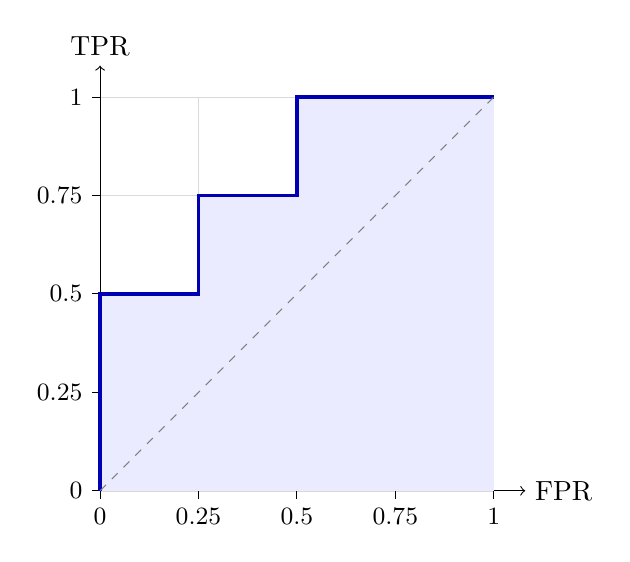
\begin{tikzpicture}[scale=5]
\rocaxes
\fill[blue!8] (0,0) -- (0,0.5) -- (0.25,0.5) -- (0.25,0.75) -- (0.5,0.75) -- (0.5,1) -- (1,1) -- (1,0) -- cycle;
\draw[very thick,blue!70!black] (0,0) -- (0,0.5) -- (0.25,0.5) -- (0.25,0.75) -- (0.5,0.75) -- (0.5,1) -- (1,1);
\draw[dashed,gray] (0,0) -- (1,1);
\end{tikzpicture}
\end{center}
\end{solution}

\part[2] Compute the AUC.
\begin{solution}
The area under the staircase, in columns of width $0.25$ with heights $0.5, 0.75, 1, 1$:
$\mathrm{AUC} = 0.25 \times (0.5 + 0.75 + 1 + 1) = 0.8125 \approx 0.81$.
\end{solution}
\end{parts}

% ===================================================================== 2
\titledquestion{Support vector machines (20 points)}
\begin{parts}
\part[10] A soft-margin SVM returned $\bm{w} = (6, 8)$, $b = -20$.
\begin{center}
\begin{tabular}{lccccc}
\toprule
point  & A & B & C & D & E \\
\midrule
$x_1$  & 3 & 1 & 1.5 & 1.25 & 3 \\
$x_2$  & 1 & 1 & 1.5 & 1.5 & 0.5 \\
label  & $+$ & $-$ & $+$ & $-$ & $-$ \\
\bottomrule
\end{tabular}
\end{center}
\begin{subparts}
\subpart Compute $f(\bm{x})$ and the predicted class of each point.
\subpart What is the width of the margin?
\subpart Compute each point's distance to the decision boundary.
\subpart Which points are support vectors? Which point is on the margin, which is inside it, and
which is misclassified?
\end{subparts}
\begin{solution}
$f(\bm{x}) = 6x_1 + 8x_2 - 20$ and $\|\bm{w}\| = \sqrt{6^2 + 8^2} = 10$.
\begin{center}
\begin{tabular}{lccccc}
\toprule
point & A & B & C & D & E \\
\midrule
$f(\bm{x})$                       & $6$   & $-6$  & $1$   & $-0.5$ & $2$ \\
predicted class                   & $+$   & $-$   & $+$   & $-$    & $+$ \\
distance $|f(\bm{x})|/\|\bm{w}\|$ & $0.6$ & $0.6$ & $0.1$ & $0.05$ & $0.2$ \\
$y\,f(\bm{x})$                    & $6$   & $6$   & $1$   & $0.5$  & $-2$ \\
\bottomrule
\end{tabular}
\end{center}
(b) Margin width $= 2/\|\bm{w}\| = 2/10 = 0.2$.

(d) The support vectors are the points with $y\,f(\bm{x}) \le 1$: C, D and E. C is on the margin
($y\,f = 1$), D is inside the margin but correctly classified ($y\,f = 0.5$), and E is
misclassified (label $-$, predicted $+$).
\end{solution}

\part[4] The soft-margin SVM solves
\[
\min_{\bm{w},\, b,\, \bm{\xi}} \ \tfrac12 \|\bm{w}\|^2 + C \sum_i \xi_i
\quad \text{subject to} \quad y_i(\bm{w} \cdot \bm{x}_i + b) \ge 1 - \xi_i,\ \ \xi_i \ge 0 .
\]
\begin{subparts}
\subpart What does the slack $\xi_i$ measure, and why do we need it?
\subpart Where does a training point lie, relative to the margin and the decision boundary, if
$\xi_i = 0$? If $0 < \xi_i < 1$? If $\xi_i > 1$?
\end{subparts}
\begin{solution}
(a) $\xi_i$ measures how far point $i$ falls short of being on its correct side, outside the margin.
Without slack, the constraints $y_i(\bm{w} \cdot \bm{x}_i + b) \ge 1$ have no solution when the
classes overlap; slack lets some points violate the margin, at a cost $C\xi_i$ each.

(b) $\xi_i = 0$: on its correct side, on or outside the margin. $0 < \xi_i < 1$: inside the margin,
but still correctly classified. $\xi_i > 1$: on the wrong side of the decision boundary
(misclassified). (At the solution $\xi_i = \max(0,\, 1 - y_i f(\bm{x}_i))$, so these are the cases
$y_i f \ge 1$, $0 < y_i f < 1$ and $y_i f < 0$.)
\end{solution}

\part[4] Two soft-margin SVMs are trained on the same data, one with $C = 0.01$ and one with
$C = 100$.
\begin{subparts}
\subpart Which has the wider margin, and why?
\subpart Which has more support vectors, and why?
\subpart Which is more likely to overfit, and why?
\subpart How would you choose $C$ in practice, and why?
\end{subparts}
\begin{solution}
(a) $C = 0.01$: slack is cheap, so the SVM accepts many points inside the margin in exchange for a
wider one.
(b) $C = 0.01$: with a wider margin, more points fall on or inside it, and all of them are support
vectors.
(c) $C = 100$: violations are expensive, so the margin narrows to fit individual training points.
(d) $C$ is a hyperparameter: try several values and pick the one with the best accuracy on
validation data (or by cross-validation). Training accuracy cannot choose it, because a larger $C$
always fits the training data at least as well; only held-out data shows which $C$ generalizes.
\end{solution}

\part[2] You remove a training point that is not a support vector and retrain the SVM. What
changes? Why?
\begin{solution}
Nothing. The solution depends only on the support vectors; a point outside the margin does not
affect $\bm{w}$ or $b$.
\end{solution}
\end{parts}

\end{questions}
\end{document}
"
\documentclass[11pt,addpoints]{exam}
\ifdefined\withsolutions \printanswers \fi
\usepackage[margin=1in]{geometry}
\usepackage{amsmath,amssymb,bm,booktabs,tikz}
\usepackage[T1]{fontenc}
\usepackage{lmodern}

% parts numbered 1.1, 1.2, ...; subparts (a), (b), ...
\renewcommand{\thepartno}{\thequestion.\arabic{partno}}
\renewcommand{\partlabel}{\thepartno}
\renewcommand{\thesubpart}{\alph{subpart}}
\renewcommand{\subpartlabel}{(\thesubpart)}
\qformat{\large\bfseries \thequestion.\ \thequestiontitle\hfill}
\pointname{ points}
\pointformat{(\thepoints)}
\bracketedpoints
\unframedsolutions
\renewcommand{\solutiontitle}{\noindent\textbf{Solution:}\enspace}

% an empty ROC plot (unit square, ticks every 0.25) for students to draw in
\newcommand{\rocaxes}{%
  \draw[step=0.25,gray!30,very thin] (0,0) grid (1,1);
  \draw[->] (0,0) -- (1.08,0) node[right] {FPR};
  \draw[->] (0,0) -- (0,1.08) node[above] {TPR};
  \foreach \t in {0,0.25,0.5,0.75,1} {
    \draw (\t,0) -- (\t,-0.02) node[below] {\small\t};
    \draw (0,\t) -- (-0.02,\t) node[left] {\small\t};}}

\begin{document}
\begin{center}
  {\Large\bfseries Machine Learning: Midterm}\\[4pt]
  \ifprintanswers Solutions \else Name: \rule{6cm}{0.4pt} \fi
\end{center}
\vspace{1em}

\begin{questions}

% ===================================================================== 1
\titledquestion{Evaluating classifiers (20 points)}
A course runs an AI-text detector on all 400 essays submitted for an assignment. An honor-code
review later established that 60 of the essays were written with AI. The detector flagged 50
essays, and 45 of the flagged essays were written with AI. Treat ``written with AI'' as the
positive class.

\begin{parts}
\part[4] Write down the confusion matrix.
\begin{solution}
60 AI-written essays and 340 human-written essays.
\begin{center}
\begin{tabular}{lcc}
\toprule
 & flagged & not flagged \\
\midrule
written with AI & TP $= 45$ & FN $= 15$ \\
human-written   & FP $= 5$  & TN $= 335$ \\
\bottomrule
\end{tabular}
\end{center}
\end{solution}

\part[2] What are precision and recall for this detector?
\begin{solution}
Precision $= 45/50 = 0.90$. \quad Recall $= 45/60 = 0.75$.
\end{solution}

\part[2] Do we care more about improving precision or recall for this problem, and why?
\begin{solution}
Precision. A false positive accuses an innocent student of cheating; a missed AI essay (false
negative) is a smaller harm. A flag should almost always be right before anyone acts on it.
\end{solution}

\uplevel{The detector also gives each essay a score between 0 and 1; a higher score means ``more
likely written with AI''. Here are 8 essays, 4 written with AI and 4 by students:
\begin{center}
\begin{tabular}{lcccccccc}
\toprule
essay            & 1 & 2 & 3 & 4 & 5 & 6 & 7 & 8 \\
\midrule
score            & 0.95 & 0.85 & 0.70 & 0.60 & 0.50 & 0.40 & 0.30 & 0.10 \\
written with AI? & yes & yes & no & yes & no & yes & no & no \\
\bottomrule
\end{tabular}
\end{center}
We say the detector flags an essay as AI-written if its score is over $t$.}

\part[10] Draw the ROC curve.
\ifprintanswers\else
\begin{center}
\begin{tikzpicture}[scale=6]\rocaxes\end{tikzpicture}
\end{center}
\fi
\begin{solution}
As $t$ passes each essay, from the highest score down, an AI essay moves the point up by
$1/4 = 0.25$ and a human essay moves it right by $0.25$. Starting at $(0,0)$, the points are
\[
(0,0.25),\ (0,0.5),\ (0.25,0.5),\ (0.25,0.75),\ (0.5,0.75),\ (0.5,1),\ (0.75,1),\ (1,1).
\]
\begin{center}
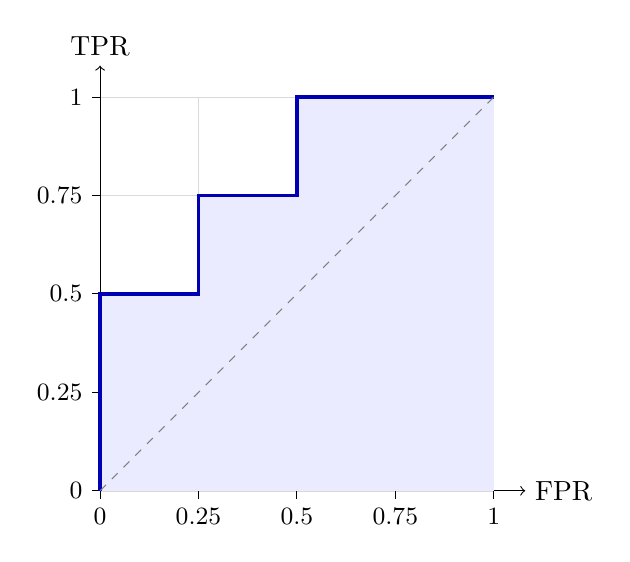
\begin{tikzpicture}[scale=5]
\rocaxes
\fill[blue!8] (0,0) -- (0,0.5) -- (0.25,0.5) -- (0.25,0.75) -- (0.5,0.75) -- (0.5,1) -- (1,1) -- (1,0) -- cycle;
\draw[very thick,blue!70!black] (0,0) -- (0,0.5) -- (0.25,0.5) -- (0.25,0.75) -- (0.5,0.75) -- (0.5,1) -- (1,1);
\draw[dashed,gray] (0,0) -- (1,1);
\end{tikzpicture}
\end{center}
\end{solution}

\part[2] Compute the AUC.
\begin{solution}
The area under the staircase, in columns of width $0.25$ with heights $0.5, 0.75, 1, 1$:
$\mathrm{AUC} = 0.25 \times (0.5 + 0.75 + 1 + 1) = 0.8125 \approx 0.81$.
\end{solution}
\end{parts}

% ===================================================================== 2
\titledquestion{Support vector machines (20 points)}
\begin{parts}
\part[10] A soft-margin SVM returned $\bm{w} = (6, 8)$, $b = -20$.
\begin{center}
\begin{tabular}{lccccc}
\toprule
point  & A & B & C & D & E \\
\midrule
$x_1$  & 3 & 1 & 1.5 & 1.25 & 3 \\
$x_2$  & 1 & 1 & 1.5 & 1.5 & 0.5 \\
label  & $+$ & $-$ & $+$ & $-$ & $-$ \\
\bottomrule
\end{tabular}
\end{center}
\begin{subparts}
\subpart Compute $f(\bm{x})$ and the predicted class of each point.
\subpart What is the width of the margin?
\subpart Compute each point's distance to the decision boundary.
\subpart Which points are support vectors? Which point is on the margin, which is inside it, and
which is misclassified?
\end{subparts}
\begin{solution}
$f(\bm{x}) = 6x_1 + 8x_2 - 20$ and $\|\bm{w}\| = \sqrt{6^2 + 8^2} = 10$.
\begin{center}
\begin{tabular}{lccccc}
\toprule
point & A & B & C & D & E \\
\midrule
$f(\bm{x})$                       & $6$   & $-6$  & $1$   & $-0.5$ & $2$ \\
predicted class                   & $+$   & $-$   & $+$   & $-$    & $+$ \\
distance $|f(\bm{x})|/\|\bm{w}\|$ & $0.6$ & $0.6$ & $0.1$ & $0.05$ & $0.2$ \\
$y\,f(\bm{x})$                    & $6$   & $6$   & $1$   & $0.5$  & $-2$ \\
\bottomrule
\end{tabular}
\end{center}
(b) Margin width $= 2/\|\bm{w}\| = 2/10 = 0.2$.

(d) The support vectors are the points with $y\,f(\bm{x}) \le 1$: C, D and E. C is on the margin
($y\,f = 1$), D is inside the margin but correctly classified ($y\,f = 0.5$), and E is
misclassified (label $-$, predicted $+$).
\end{solution}

\part[4] The soft-margin SVM solves
\[
\min_{\bm{w},\, b,\, \bm{\xi}} \ \tfrac12 \|\bm{w}\|^2 + C \sum_i \xi_i
\quad \text{subject to} \quad y_i(\bm{w} \cdot \bm{x}_i + b) \ge 1 - \xi_i,\ \ \xi_i \ge 0 .
\]
\begin{subparts}
\subpart What does the slack $\xi_i$ measure, and why do we need it?
\subpart Where does a training point lie, relative to the margin and the decision boundary, if
$\xi_i = 0$? If $0 < \xi_i < 1$? If $\xi_i > 1$?
\end{subparts}
\begin{solution}
(a) $\xi_i$ measures how far point $i$ falls short of being on its correct side, outside the margin.
Without slack, the constraints $y_i(\bm{w} \cdot \bm{x}_i + b) \ge 1$ have no solution when the
classes overlap; slack lets some points violate the margin, at a cost $C\xi_i$ each.

(b) $\xi_i = 0$: on its correct side, on or outside the margin. $0 < \xi_i < 1$: inside the margin,
but still correctly classified. $\xi_i > 1$: on the wrong side of the decision boundary
(misclassified). (At the solution $\xi_i = \max(0,\, 1 - y_i f(\bm{x}_i))$, so these are the cases
$y_i f \ge 1$, $0 < y_i f < 1$ and $y_i f < 0$.)
\end{solution}

\part[4] Two soft-margin SVMs are trained on the same data, one with $C = 0.01$ and one with
$C = 100$.
\begin{subparts}
\subpart Which has the wider margin, and why?
\subpart Which has more support vectors, and why?
\subpart Which is more likely to overfit, and why?
\subpart How would you choose $C$ in practice, and why?
\end{subparts}
\begin{solution}
(a) $C = 0.01$: slack is cheap, so the SVM accepts many points inside the margin in exchange for a
wider one.
(b) $C = 0.01$: with a wider margin, more points fall on or inside it, and all of them are support
vectors.
(c) $C = 100$: violations are expensive, so the margin narrows to fit individual training points.
(d) $C$ is a hyperparameter: try several values and pick the one with the best accuracy on
validation data (or by cross-validation). Training accuracy cannot choose it, because a larger $C$
always fits the training data at least as well; only held-out data shows which $C$ generalizes.
\end{solution}

\part[2] You remove a training point that is not a support vector and retrain the SVM. What
changes? Why?
\begin{solution}
Nothing. The solution depends only on the support vectors; a point outside the margin does not
affect $\bm{w}$ or $b$.
\end{solution}
\end{parts}

\end{questions}
\end{document}
"
\documentclass[11pt,addpoints]{exam}
\ifdefined\withsolutions \printanswers \fi
\usepackage[margin=1in]{geometry}
\usepackage{amsmath,amssymb,bm,booktabs,tikz}
\usepackage[T1]{fontenc}
\usepackage{lmodern}

% parts numbered 1.1, 1.2, ...; subparts (a), (b), ...
\renewcommand{\thepartno}{\thequestion.\arabic{partno}}
\renewcommand{\partlabel}{\thepartno}
\renewcommand{\thesubpart}{\alph{subpart}}
\renewcommand{\subpartlabel}{(\thesubpart)}
\qformat{\large\bfseries \thequestion.\ \thequestiontitle\hfill}
\pointname{ points}
\pointformat{(\thepoints)}
\bracketedpoints
\unframedsolutions
\renewcommand{\solutiontitle}{\noindent\textbf{Solution:}\enspace}

% an empty ROC plot (unit square, ticks every 0.25) for students to draw in
\newcommand{\rocaxes}{%
  \draw[step=0.25,gray!30,very thin] (0,0) grid (1,1);
  \draw[->] (0,0) -- (1.08,0) node[right] {FPR};
  \draw[->] (0,0) -- (0,1.08) node[above] {TPR};
  \foreach \t in {0,0.25,0.5,0.75,1} {
    \draw (\t,0) -- (\t,-0.02) node[below] {\small\t};
    \draw (0,\t) -- (-0.02,\t) node[left] {\small\t};}}

\begin{document}
\begin{center}
  {\Large\bfseries Machine Learning: Midterm}\\[4pt]
  \ifprintanswers Solutions \else Name: \rule{6cm}{0.4pt} \fi
\end{center}
\vspace{1em}

\begin{questions}

% ===================================================================== 1
\titledquestion{Evaluating classifiers (20 points)}
A course runs an AI-text detector on all 400 essays submitted for an assignment. An honor-code
review later established that 60 of the essays were written with AI. The detector flagged 50
essays, and 45 of the flagged essays were written with AI. Treat ``written with AI'' as the
positive class.

\begin{parts}
\part[4] Write down the confusion matrix.
\begin{solution}
60 AI-written essays and 340 human-written essays.
\begin{center}
\begin{tabular}{lcc}
\toprule
 & flagged & not flagged \\
\midrule
written with AI & TP $= 45$ & FN $= 15$ \\
human-written   & FP $= 5$  & TN $= 335$ \\
\bottomrule
\end{tabular}
\end{center}
\end{solution}

\part[2] What are precision and recall for this detector?
\begin{solution}
Precision $= 45/50 = 0.90$. \quad Recall $= 45/60 = 0.75$.
\end{solution}

\part[2] Do we care more about improving precision or recall for this problem, and why?
\begin{solution}
Precision. A false positive accuses an innocent student of cheating; a missed AI essay (false
negative) is a smaller harm. A flag should almost always be right before anyone acts on it.
\end{solution}

\uplevel{The detector also gives each essay a score between 0 and 1; a higher score means ``more
likely written with AI''. Here are 8 essays, 4 written with AI and 4 by students:
\begin{center}
\begin{tabular}{lcccccccc}
\toprule
essay            & 1 & 2 & 3 & 4 & 5 & 6 & 7 & 8 \\
\midrule
score            & 0.95 & 0.85 & 0.70 & 0.60 & 0.50 & 0.40 & 0.30 & 0.10 \\
written with AI? & yes & yes & no & yes & no & yes & no & no \\
\bottomrule
\end{tabular}
\end{center}
We say the detector flags an essay as AI-written if its score is over $t$.}

\part[10] Draw the ROC curve.
\ifprintanswers\else
\begin{center}
\begin{tikzpicture}[scale=6]\rocaxes\end{tikzpicture}
\end{center}
\fi
\begin{solution}
As $t$ passes each essay, from the highest score down, an AI essay moves the point up by
$1/4 = 0.25$ and a human essay moves it right by $0.25$. Starting at $(0,0)$, the points are
\[
(0,0.25),\ (0,0.5),\ (0.25,0.5),\ (0.25,0.75),\ (0.5,0.75),\ (0.5,1),\ (0.75,1),\ (1,1).
\]
\begin{center}
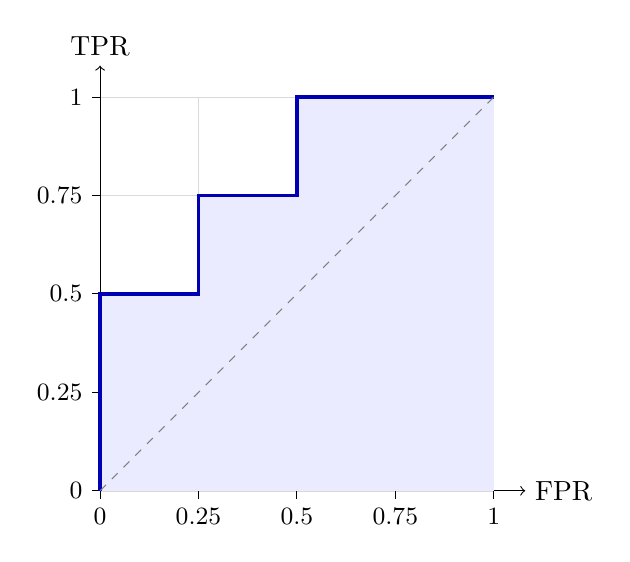
\begin{tikzpicture}[scale=5]
\rocaxes
\fill[blue!8] (0,0) -- (0,0.5) -- (0.25,0.5) -- (0.25,0.75) -- (0.5,0.75) -- (0.5,1) -- (1,1) -- (1,0) -- cycle;
\draw[very thick,blue!70!black] (0,0) -- (0,0.5) -- (0.25,0.5) -- (0.25,0.75) -- (0.5,0.75) -- (0.5,1) -- (1,1);
\draw[dashed,gray] (0,0) -- (1,1);
\end{tikzpicture}
\end{center}
\end{solution}

\part[2] Compute the AUC.
\begin{solution}
The area under the staircase, in columns of width $0.25$ with heights $0.5, 0.75, 1, 1$:
$\mathrm{AUC} = 0.25 \times (0.5 + 0.75 + 1 + 1) = 0.8125 \approx 0.81$.
\end{solution}
\end{parts}

% ===================================================================== 2
\titledquestion{Support vector machines (20 points)}
\begin{parts}
\part[10] A soft-margin SVM returned $\bm{w} = (6, 8)$, $b = -20$.
\begin{center}
\begin{tabular}{lccccc}
\toprule
point  & A & B & C & D & E \\
\midrule
$x_1$  & 3 & 1 & 1.5 & 1.25 & 3 \\
$x_2$  & 1 & 1 & 1.5 & 1.5 & 0.5 \\
label  & $+$ & $-$ & $+$ & $-$ & $-$ \\
\bottomrule
\end{tabular}
\end{center}
\begin{subparts}
\subpart Compute $f(\bm{x})$ and the predicted class of each point.
\subpart What is the width of the margin?
\subpart Compute each point's distance to the decision boundary.
\subpart Which points are support vectors? Which point is on the margin, which is inside it, and
which is misclassified?
\end{subparts}
\begin{solution}
$f(\bm{x}) = 6x_1 + 8x_2 - 20$ and $\|\bm{w}\| = \sqrt{6^2 + 8^2} = 10$.
\begin{center}
\begin{tabular}{lccccc}
\toprule
point & A & B & C & D & E \\
\midrule
$f(\bm{x})$                       & $6$   & $-6$  & $1$   & $-0.5$ & $2$ \\
predicted class                   & $+$   & $-$   & $+$   & $-$    & $+$ \\
distance $|f(\bm{x})|/\|\bm{w}\|$ & $0.6$ & $0.6$ & $0.1$ & $0.05$ & $0.2$ \\
$y\,f(\bm{x})$                    & $6$   & $6$   & $1$   & $0.5$  & $-2$ \\
\bottomrule
\end{tabular}
\end{center}
(b) Margin width $= 2/\|\bm{w}\| = 2/10 = 0.2$.

(d) The support vectors are the points with $y\,f(\bm{x}) \le 1$: C, D and E. C is on the margin
($y\,f = 1$), D is inside the margin but correctly classified ($y\,f = 0.5$), and E is
misclassified (label $-$, predicted $+$).
\end{solution}

\part[4] The soft-margin SVM solves
\[
\min_{\bm{w},\, b,\, \bm{\xi}} \ \tfrac12 \|\bm{w}\|^2 + C \sum_i \xi_i
\quad \text{subject to} \quad y_i(\bm{w} \cdot \bm{x}_i + b) \ge 1 - \xi_i,\ \ \xi_i \ge 0 .
\]
\begin{subparts}
\subpart What does the slack $\xi_i$ measure, and why do we need it?
\subpart Where does a training point lie, relative to the margin and the decision boundary, if
$\xi_i = 0$? If $0 < \xi_i < 1$? If $\xi_i > 1$?
\end{subparts}
\begin{solution}
(a) $\xi_i$ measures how far point $i$ falls short of being on its correct side, outside the margin.
Without slack, the constraints $y_i(\bm{w} \cdot \bm{x}_i + b) \ge 1$ have no solution when the
classes overlap; slack lets some points violate the margin, at a cost $C\xi_i$ each.

(b) $\xi_i = 0$: on its correct side, on or outside the margin. $0 < \xi_i < 1$: inside the margin,
but still correctly classified. $\xi_i > 1$: on the wrong side of the decision boundary
(misclassified). (At the solution $\xi_i = \max(0,\, 1 - y_i f(\bm{x}_i))$, so these are the cases
$y_i f \ge 1$, $0 < y_i f < 1$ and $y_i f < 0$.)
\end{solution}

\part[4] Two soft-margin SVMs are trained on the same data, one with $C = 0.01$ and one with
$C = 100$.
\begin{subparts}
\subpart Which has the wider margin, and why?
\subpart Which has more support vectors, and why?
\subpart Which is more likely to overfit, and why?
\subpart How would you choose $C$ in practice, and why?
\end{subparts}
\begin{solution}
(a) $C = 0.01$: slack is cheap, so the SVM accepts many points inside the margin in exchange for a
wider one.
(b) $C = 0.01$: with a wider margin, more points fall on or inside it, and all of them are support
vectors.
(c) $C = 100$: violations are expensive, so the margin narrows to fit individual training points.
(d) $C$ is a hyperparameter: try several values and pick the one with the best accuracy on
validation data (or by cross-validation). Training accuracy cannot choose it, because a larger $C$
always fits the training data at least as well; only held-out data shows which $C$ generalizes.
\end{solution}

\part[2] You remove a training point that is not a support vector and retrain the SVM. What
changes? Why?
\begin{solution}
Nothing. The solution depends only on the support vectors; a point outside the margin does not
affect $\bm{w}$ or $b$.
\end{solution}
\end{parts}

\end{questions}
\end{document}
"
\documentclass[11pt,addpoints]{exam}
\ifdefined\withsolutions \printanswers \fi
\usepackage[margin=1in]{geometry}
\usepackage{amsmath,amssymb,bm,booktabs,tikz}
\usepackage[T1]{fontenc}
\usepackage{lmodern}

% parts numbered 1.1, 1.2, ...; subparts (a), (b), ...
\renewcommand{\thepartno}{\thequestion.\arabic{partno}}
\renewcommand{\partlabel}{\thepartno}
\renewcommand{\thesubpart}{\alph{subpart}}
\renewcommand{\subpartlabel}{(\thesubpart)}
\qformat{\large\bfseries \thequestion.\ \thequestiontitle\hfill}
\pointname{ points}
\pointformat{(\thepoints)}
\bracketedpoints
\unframedsolutions
\renewcommand{\solutiontitle}{\noindent\textbf{Solution:}\enspace}

% an empty ROC plot (unit square, ticks every 0.25) for students to draw in
\newcommand{\rocaxes}{%
  \draw[step=0.25,gray!30,very thin] (0,0) grid (1,1);
  \draw[->] (0,0) -- (1.08,0) node[right] {FPR};
  \draw[->] (0,0) -- (0,1.08) node[above] {TPR};
  \foreach \t in {0,0.25,0.5,0.75,1} {
    \draw (\t,0) -- (\t,-0.02) node[below] {\small\t};
    \draw (0,\t) -- (-0.02,\t) node[left] {\small\t};}}

\begin{document}
\begin{center}
  {\Large\bfseries Machine Learning: Midterm}\\[4pt]
  \ifprintanswers Solutions \else Name: \rule{6cm}{0.4pt} \fi
\end{center}
\vspace{1em}

\begin{questions}

% ===================================================================== 1
\titledquestion{Evaluating classifiers (20 points)}
A course runs an AI-text detector on all 400 essays submitted for an assignment. An honor-code
review later established that 60 of the essays were written with AI. The detector flagged 50
essays, and 45 of the flagged essays were written with AI. Treat ``written with AI'' as the
positive class.

\begin{parts}
\part[4] Write down the confusion matrix.
\begin{solution}
60 AI-written essays and 340 human-written essays.
\begin{center}
\begin{tabular}{lcc}
\toprule
 & flagged & not flagged \\
\midrule
written with AI & TP $= 45$ & FN $= 15$ \\
human-written   & FP $= 5$  & TN $= 335$ \\
\bottomrule
\end{tabular}
\end{center}
\end{solution}

\part[2] What are precision and recall for this detector?
\begin{solution}
Precision $= 45/50 = 0.90$. \quad Recall $= 45/60 = 0.75$.
\end{solution}

\part[2] Do we care more about improving precision or recall for this problem, and why?
\begin{solution}
Precision. A false positive accuses an innocent student of cheating; a missed AI essay (false
negative) is a smaller harm. A flag should almost always be right before anyone acts on it.
\end{solution}

\uplevel{The detector also gives each essay a score between 0 and 1; a higher score means ``more
likely written with AI''. Here are 8 essays, 4 written with AI and 4 by students:
\begin{center}
\begin{tabular}{lcccccccc}
\toprule
essay            & 1 & 2 & 3 & 4 & 5 & 6 & 7 & 8 \\
\midrule
score            & 0.95 & 0.85 & 0.70 & 0.60 & 0.50 & 0.40 & 0.30 & 0.10 \\
written with AI? & yes & yes & no & yes & no & yes & no & no \\
\bottomrule
\end{tabular}
\end{center}
We say the detector flags an essay as AI-written if its score is over $t$.}

\part[10] Draw the ROC curve.
\ifprintanswers\else
\begin{center}
\begin{tikzpicture}[scale=6]\rocaxes\end{tikzpicture}
\end{center}
\fi
\begin{solution}
As $t$ passes each essay, from the highest score down, an AI essay moves the point up by
$1/4 = 0.25$ and a human essay moves it right by $0.25$. Starting at $(0,0)$, the points are
\[
(0,0.25),\ (0,0.5),\ (0.25,0.5),\ (0.25,0.75),\ (0.5,0.75),\ (0.5,1),\ (0.75,1),\ (1,1).
\]
\begin{center}
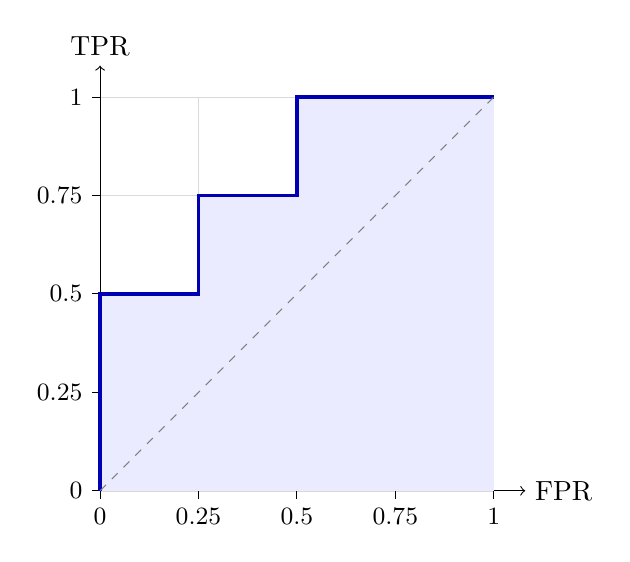
\begin{tikzpicture}[scale=5]
\rocaxes
\fill[blue!8] (0,0) -- (0,0.5) -- (0.25,0.5) -- (0.25,0.75) -- (0.5,0.75) -- (0.5,1) -- (1,1) -- (1,0) -- cycle;
\draw[very thick,blue!70!black] (0,0) -- (0,0.5) -- (0.25,0.5) -- (0.25,0.75) -- (0.5,0.75) -- (0.5,1) -- (1,1);
\draw[dashed,gray] (0,0) -- (1,1);
\end{tikzpicture}
\end{center}
\end{solution}

\part[2] Compute the AUC.
\begin{solution}
The area under the staircase, in columns of width $0.25$ with heights $0.5, 0.75, 1, 1$:
$\mathrm{AUC} = 0.25 \times (0.5 + 0.75 + 1 + 1) = 0.8125 \approx 0.81$.
\end{solution}
\end{parts}

% ===================================================================== 2
\titledquestion{Support vector machines (20 points)}
\begin{parts}
\part[10] A soft-margin SVM returned $\bm{w} = (6, 8)$, $b = -20$.
\begin{center}
\begin{tabular}{lccccc}
\toprule
point  & A & B & C & D & E \\
\midrule
$x_1$  & 3 & 1 & 1.5 & 1.25 & 3 \\
$x_2$  & 1 & 1 & 1.5 & 1.5 & 0.5 \\
label  & $+$ & $-$ & $+$ & $-$ & $-$ \\
\bottomrule
\end{tabular}
\end{center}
\begin{subparts}
\subpart Compute $f(\bm{x})$ and the predicted class of each point.
\subpart What is the width of the margin?
\subpart Compute each point's distance to the decision boundary.
\subpart Which points are support vectors? Which point is on the margin, which is inside it, and
which is misclassified?
\end{subparts}
\begin{solution}
$f(\bm{x}) = 6x_1 + 8x_2 - 20$ and $\|\bm{w}\| = \sqrt{6^2 + 8^2} = 10$.
\begin{center}
\begin{tabular}{lccccc}
\toprule
point & A & B & C & D & E \\
\midrule
$f(\bm{x})$                       & $6$   & $-6$  & $1$   & $-0.5$ & $2$ \\
predicted class                   & $+$   & $-$   & $+$   & $-$    & $+$ \\
distance $|f(\bm{x})|/\|\bm{w}\|$ & $0.6$ & $0.6$ & $0.1$ & $0.05$ & $0.2$ \\
$y\,f(\bm{x})$                    & $6$   & $6$   & $1$   & $0.5$  & $-2$ \\
\bottomrule
\end{tabular}
\end{center}
(b) Margin width $= 2/\|\bm{w}\| = 2/10 = 0.2$.

(d) The support vectors are the points with $y\,f(\bm{x}) \le 1$: C, D and E. C is on the margin
($y\,f = 1$), D is inside the margin but correctly classified ($y\,f = 0.5$), and E is
misclassified (label $-$, predicted $+$).
\end{solution}

\part[4] The soft-margin SVM solves
\[
\min_{\bm{w},\, b,\, \bm{\xi}} \ \tfrac12 \|\bm{w}\|^2 + C \sum_i \xi_i
\quad \text{subject to} \quad y_i(\bm{w} \cdot \bm{x}_i + b) \ge 1 - \xi_i,\ \ \xi_i \ge 0 .
\]
\begin{subparts}
\subpart What does the slack $\xi_i$ measure, and why do we need it?
\subpart Where does a training point lie, relative to the margin and the decision boundary, if
$\xi_i = 0$? If $0 < \xi_i < 1$? If $\xi_i > 1$?
\end{subparts}
\begin{solution}
(a) $\xi_i$ measures how far point $i$ falls short of being on its correct side, outside the margin.
Without slack, the constraints $y_i(\bm{w} \cdot \bm{x}_i + b) \ge 1$ have no solution when the
classes overlap; slack lets some points violate the margin, at a cost $C\xi_i$ each.

(b) $\xi_i = 0$: on its correct side, on or outside the margin. $0 < \xi_i < 1$: inside the margin,
but still correctly classified. $\xi_i > 1$: on the wrong side of the decision boundary
(misclassified). (At the solution $\xi_i = \max(0,\, 1 - y_i f(\bm{x}_i))$, so these are the cases
$y_i f \ge 1$, $0 < y_i f < 1$ and $y_i f < 0$.)
\end{solution}

\part[4] Two soft-margin SVMs are trained on the same data, one with $C = 0.01$ and one with
$C = 100$.
\begin{subparts}
\subpart Which has the wider margin, and why?
\subpart Which has more support vectors, and why?
\subpart Which is more likely to overfit, and why?
\subpart How would you choose $C$ in practice, and why?
\end{subparts}
\begin{solution}
(a) $C = 0.01$: slack is cheap, so the SVM accepts many points inside the margin in exchange for a
wider one.
(b) $C = 0.01$: with a wider margin, more points fall on or inside it, and all of them are support
vectors.
(c) $C = 100$: violations are expensive, so the margin narrows to fit individual training points.
(d) $C$ is a hyperparameter: try several values and pick the one with the best accuracy on
validation data (or by cross-validation). Training accuracy cannot choose it, because a larger $C$
always fits the training data at least as well; only held-out data shows which $C$ generalizes.
\end{solution}

\part[2] You remove a training point that is not a support vector and retrain the SVM. What
changes? Why?
\begin{solution}
Nothing. The solution depends only on the support vectors; a point outside the margin does not
affect $\bm{w}$ or $b$.
\end{solution}
\end{parts}

\end{questions}
\end{document}
